% ----------------------------------------------------------------
% Article Class (This is a LaTeX2e document)  ********************
% ----------------------------------------------------------------
\documentclass[11pt]{article}
\usepackage[english]{babel}
\usepackage{amsmath,amsthm, amssymb}
\usepackage{amsfonts}
\usepackage{multirow}
\usepackage{threeparttable}

%Candelaria's favorite packages
\usepackage{setspace}	% Set the spacing for the document
\usepackage{xtab}		% Use for tables
\usepackage{comment}	% Use for block comments
\usepackage{rotating}	% Helpful for rotating figures
\usepackage{lscape}	% Change a page into landscape
\usepackage{hyperref}
\hypersetup{colorlinks=false,pdfborder={0 0 0},breaklinks=true}
\usepackage{graphicx}	% Load a graphic image
%\usepackage{url}		% Use for formatting URLS (nice for NatBib also)
\usepackage{booktabs}  	% Use for nice tables/ Works well with ESTOUT
\usepackage{longtable} 	% Used to break long tables over multiple pages
\usepackage{caption}
\usepackage{subcaption} 	% Used to create SubFloats
\usepackage{listings} 	% Use to enter code blocks, like a fancy verbatim
\usepackage{enumerate}
% ADD COLOR:
\usepackage{color}
\usepackage[usenames, dvipsnames, svgnames, table]{xcolor}

% Packages for the bibliography
\usepackage[longnamesfirst]{natbib}
%\usepackage{natbib}

% Set Page Margins
%\usepackage{fullpage}
\addtolength{\oddsidemargin}{-.875in}
\addtolength{\evensidemargin}{-.875in}
\addtolength{\textwidth}{1.75in}
\addtolength{\topmargin}{-.875in}
\addtolength{\textheight}{1.75in}

% Set line and table spacing
\renewcommand{\baselinestretch}{1.0}
\renewcommand{\arraystretch}{1.1}
\setlength\abovedisplayskip{0pt}
\setlength\belowdisplayskip{0pt}

% Redefine the cite command
\renewcommand\cite{\citet}

%\setlength{\parindent}{0in}

%\setlength{\leftmargin}{0pt} \setlength{\parskip}{1.1ex} \setlength{\parindent}{1em} \setlength{\itemsep}{0pt} \setlength{\footnotesep}{10pt}
%\renewcommand{\footnoterule}{\rule{3in}{.3pt}\vspace{-.3pt}}

% THEOREMS -------------------------------------------------------
\newtheorem{thm}{Theorem}[section]
\newtheorem{cor}[thm]{Corollary}
\newtheorem{lem}[thm]{Lemma}
\newtheorem{prop}[thm]{Proposition}
\theoremstyle{definition}
\newtheorem{defn}[thm]{Definition}
\theoremstyle{remark}
\newtheorem{rem}[thm]{Remark}
%\numberwithin{equation}{section} %Number equations within section
% ----------------------------------------------------------------

%%%%%%TYPESET LINEAR EQUATIONS
\usepackage{environ}

\makeatletter

\newcommand{\LinearSystems@SetupLets}{%
  \let\col=&%
  \let\+=+%
  \let\-=-%
  \let\===%
}
\newcommand{\LinearSystems@SetupCatcodes}{%
  \catcode`\&=\active
  \catcode`\+=\active
  \catcode`\-=\active
  \catcode`\==\active
}
\newcommand{\LinearSystems@Setup}{}
\begingroup
  \LinearSystems@SetupCatcodes
  \gdef\LinearSystems@Setup{%
    \LinearSystems@SetupLets
    \LinearSystems@SetupCatcodes
    \newcommand&[1][0pt]{\col\hspace{##1}\col}%
    \def+{\col\+{}{}\col}%
    \def-{\col\-{}{}\col}%
    \def={\col\={}{}\col}%
  }
\endgroup

\NewEnviron{LinearSystems}[1]{\begin{alignat*}{#1}\BODY\end{alignat*}}
\let\LinearSystems@OriginalBegin\LinearSystems
\def\LinearSystems{\LinearSystems@Setup\LinearSystems@OriginalBegin}

\makeatother


%%%%%%%%%%%%%%%%%%%%%%%%%%%
%% COMMANDS FOR JUSTIFYING MATRIX ELEMENTS AND FOR CREATING
%% AUGMENTED MATRICES
% The following code redefines the matrix environment, such
% that we can left or right justify the contents in a matrix 

\makeatletter
\renewcommand*\env@matrix[1][*\c@MaxMatrixCols c]{%
  \hskip -\arraycolsep
  \let\@ifnextchar\new@ifnextchar
  \array{#1}}
\makeatother
%%%%%%%%%%%%%%%%%%%%%%%%

% Commands for the differential in integration
\newcommand*\diff{\mathop{}\!\mathrm{d}}
\newcommand*\Diff[1]{\mathop{}\!\mathrm{d^#1}}

\begin{document}

\begin{center}
{\huge Calculus Lecture Notes\footnote{Contributor(s): Chris Candelaria, Erin Fahle, June John and Klint Kanopka. If you find errors, please let Klint know so that he may correct them. Thanks!}} \\[5pt]
{\Large Stanford GSE Math Camp 2019 \\[5pt]
Do Not Distribute Outside GSE}
\end{center}

\section{Motivation}

Calculus can be divided into two main branches: differential and integral calculus. It pertains to the study of (infinitesimal) change. The use of calculus spans a variety of disciplines including economics; for example, for optimization. Thus, it can be helpful to remember these fundamentals, as several courses (e.g. the 102 Econ sequence or 202N Econ) assume working knowledge of calculus.

\section{Differentiation}
\begin{itemize}
\item Our goal will be to find the rate of change of one quantity compared to another
\item \textbf{Key definitions/notations:} 
\begin{itemize}
\item Slope: the concept of slope as rate of change is important. For a straight line, the slope is \begin{center} {\LARGE $\frac{\text{rise}}{\text{run}} $} = {\LARGE $\frac{\text{change in y}}{\text{change in x}} $} = {\LARGE
$\frac{\Delta{y}}{\Delta{x}}$ }\end{center}
However, for other functions, the slope will not be constant. Therefore, we use the derivative of the function.
\item Derivative: can be thought of as the slope of a tangent line at a point on a function. The derivative tells you the rate of change at a point. It is denoted by {\LARGE $ \frac{\textit{dy}}{\textit{dx}}$} or f'(x) or y'. The value of the derivative may change for different values of x. In the graph below, we see that the derivative of function f(x) is positive, then 0, then negative (from left to right). 

\end{itemize}
\begin{center}
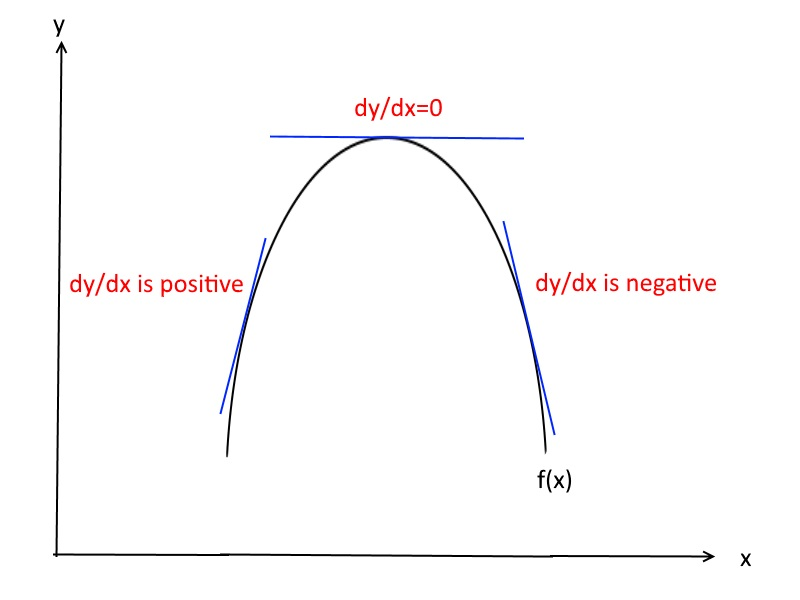
\includegraphics[scale=0.5]{img/calculus_differential1.jpg}\\
\end{center}

Consider the graph below. The derivative can be thought of as a limit of the difference in f(x) between a point of interest \textit{a} and another point, \textit{a+h}. A line through these two points is a secant with a slope, or the difference quotient: \begin{center}\LARGE{$\frac{f(a+h)-f(a)}{a+h-a} = \frac{f(a+h)-f(a)}{h}$} \end{center} 
As \textit{h} gets smaller, this equation approximates the slope of a tangent at point \textit{a}, the derivative of f(x) at point \textit{a}. This will yield the derivative, as denoted below.\\ 
\begin{center}\LARGE{$\lim_{\Delta h\rightarrow 0}\frac{f(x+h)-f(x)}{h}$} \end{center}
\begin{center}
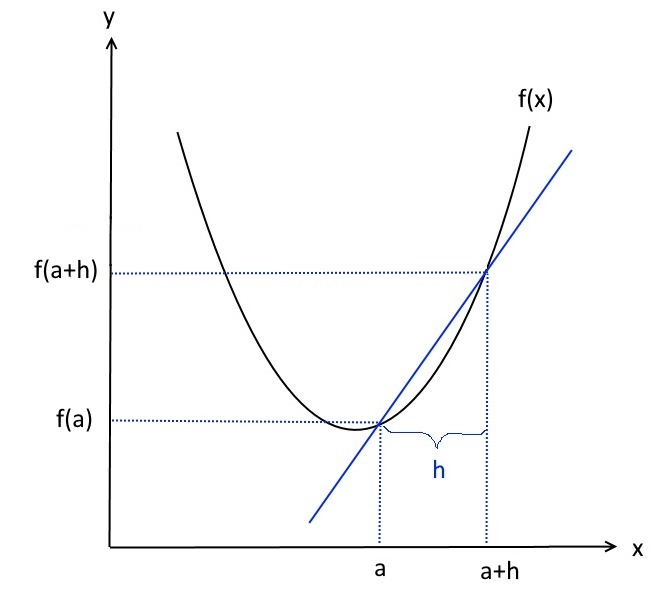
\includegraphics[scale=0.5]{img/calculus_diffquotient.jpg}\\
\end{center}
\item \textbf{Common differentiation rules}\\
\begin{enumerate}
\item $(af)'=a(f')$\\
\item $(f+g)'=f'+ g'$\\
\item $(f-g)'=f'- g'$\\
\item Product rule for $h(x)=f(x)g(x):  h'(x)=f'(x)g(x) + f(x)g'(x)$\\
\item Chain rule for $h(x)=f(g(x)): h'(x)=f'(g(x))g'(x)$\\
\item Exponents: If $f(x)=x^n$ then $f'(x)=nx^{n-1}$ and when n=0, f'(x)=0\\
\item Log rules: $\frac{d}{dx} ln\;x = \frac{1}{x}$ and $\frac{d}{dx}e^{cx}=ce^{cx}$
\\
\end{enumerate}
\end{itemize}

\section{Integration: Introduction}
\begin{itemize}
\item Our goal will be to find the area of a region $S$ that lies under the curve $f(x)$ from points $a$ to $b$.
\item Suppose our function of interest is $f(x) = x^2 + 1$ on $x\in[0,2]$. Let's define the shaded region under $f(x)$ as $S$. \\
\begin{center}
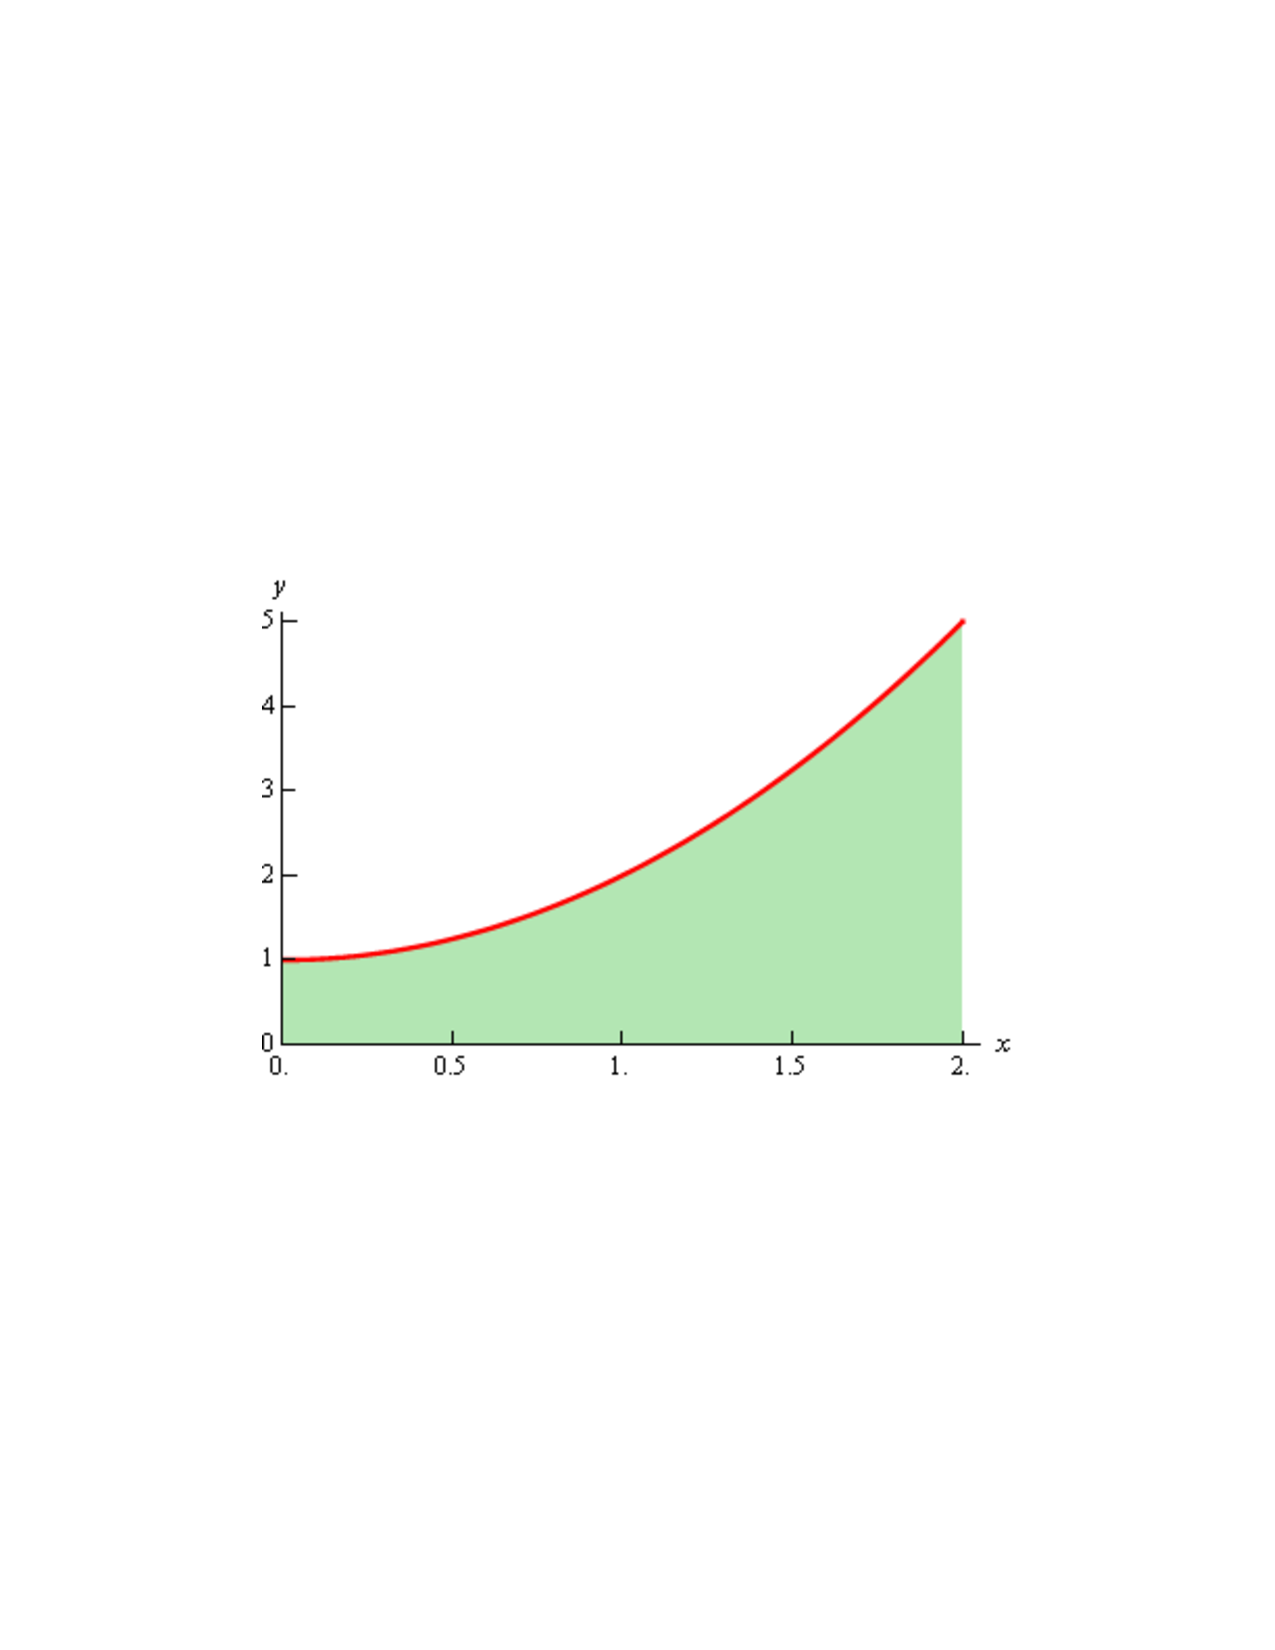
\includegraphics[scale=0.5]{img/integrals_mainfunction.pdf}\\
\end{center}
How can we find the area of $S$? We have a few options:
\begin{enumerate}
\item Rectangle method using right-hand endpoints: \\
\begin{center}
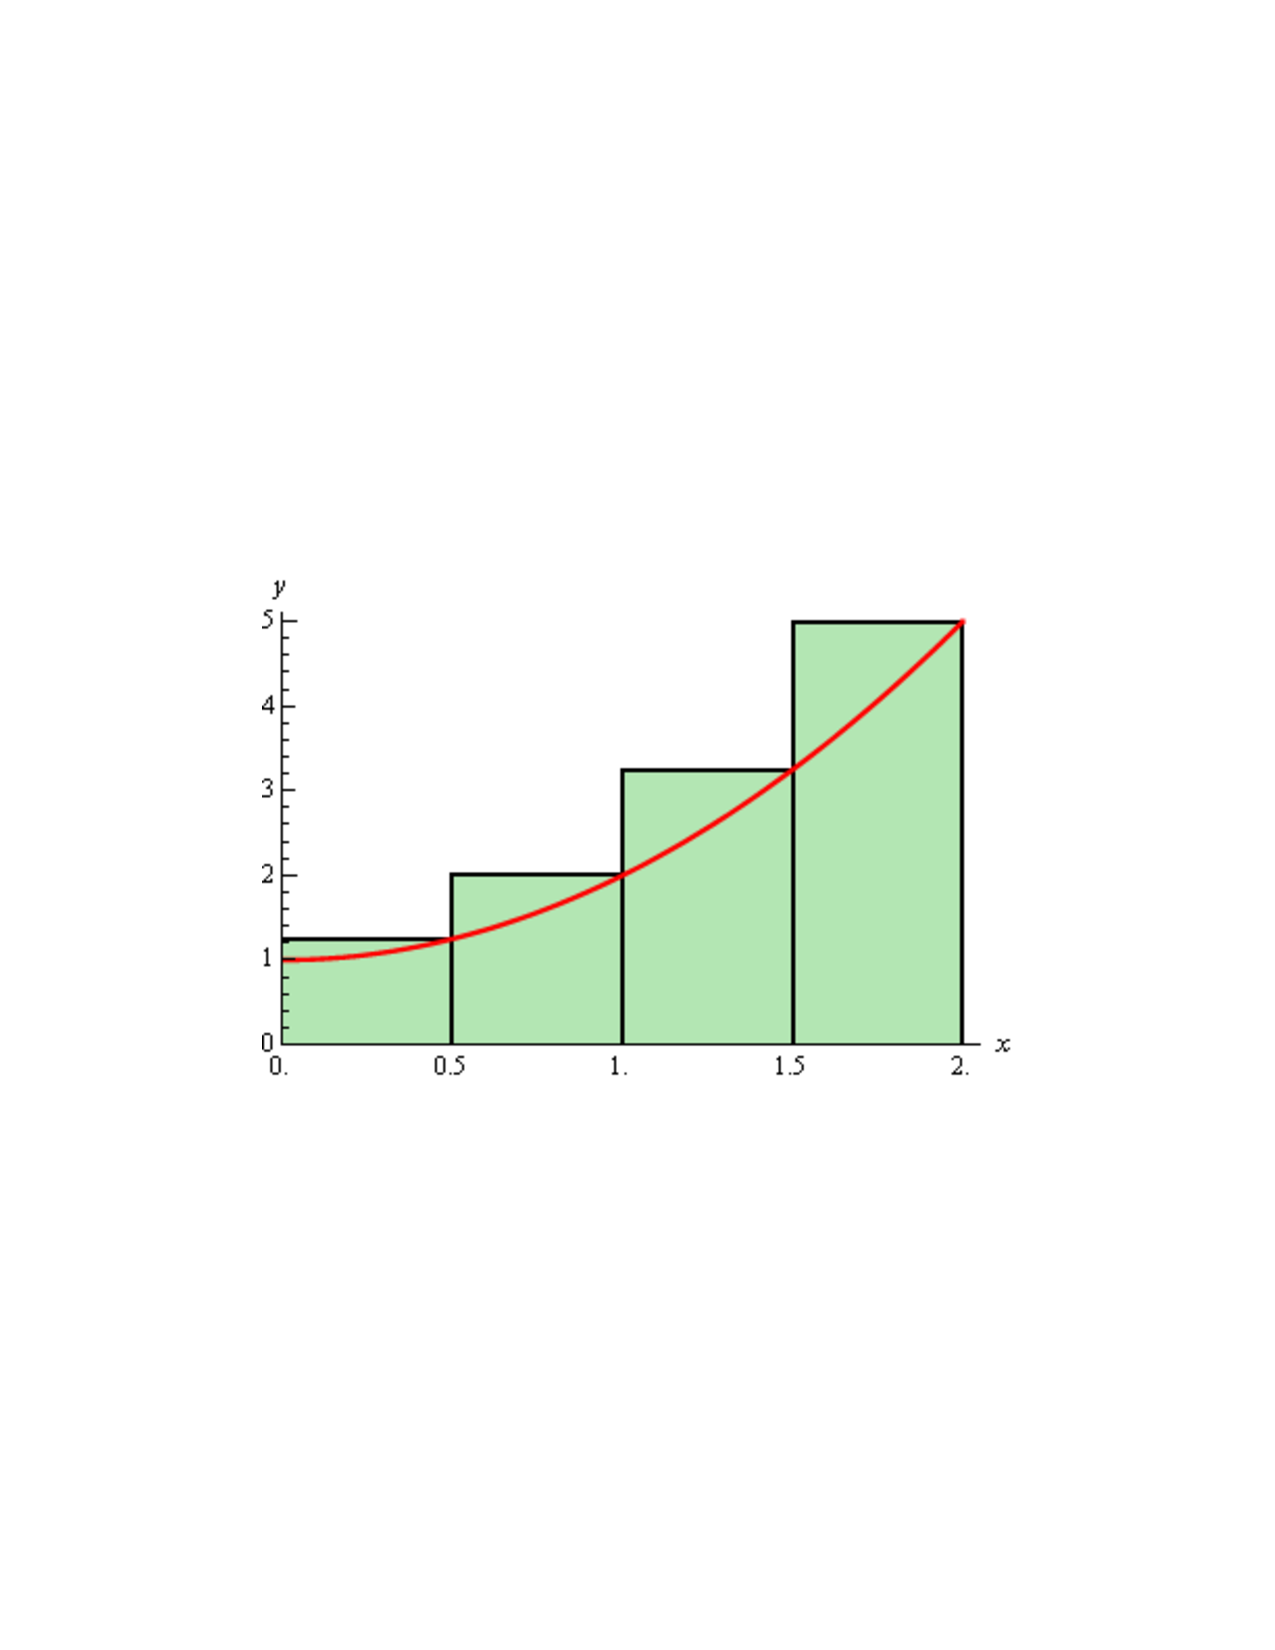
\includegraphics[scale=0.5]{img/integrals_rectangleR.pdf}
\end{center}
\begin{align*}
Area(S) &= \frac{1}{2}f\left(\frac{1}{2}\right) + \frac{1}{2}f\left(1\right) + \frac{1}{2}f\left(\frac{3}{2}\right) + \frac{1}{2}f\left(2\right) \\
&= \frac{1}{2}\left(\frac{5}{4}\right) + \frac{1}{2}\left(2\right) + \frac{1}{2}\left(\frac{13}{4}\right) + \frac{1}{2}\left(5\right) \\
&= 5.75
\end{align*}
\item Rectangle method using left-hand endpoints: \\
\begin{center}
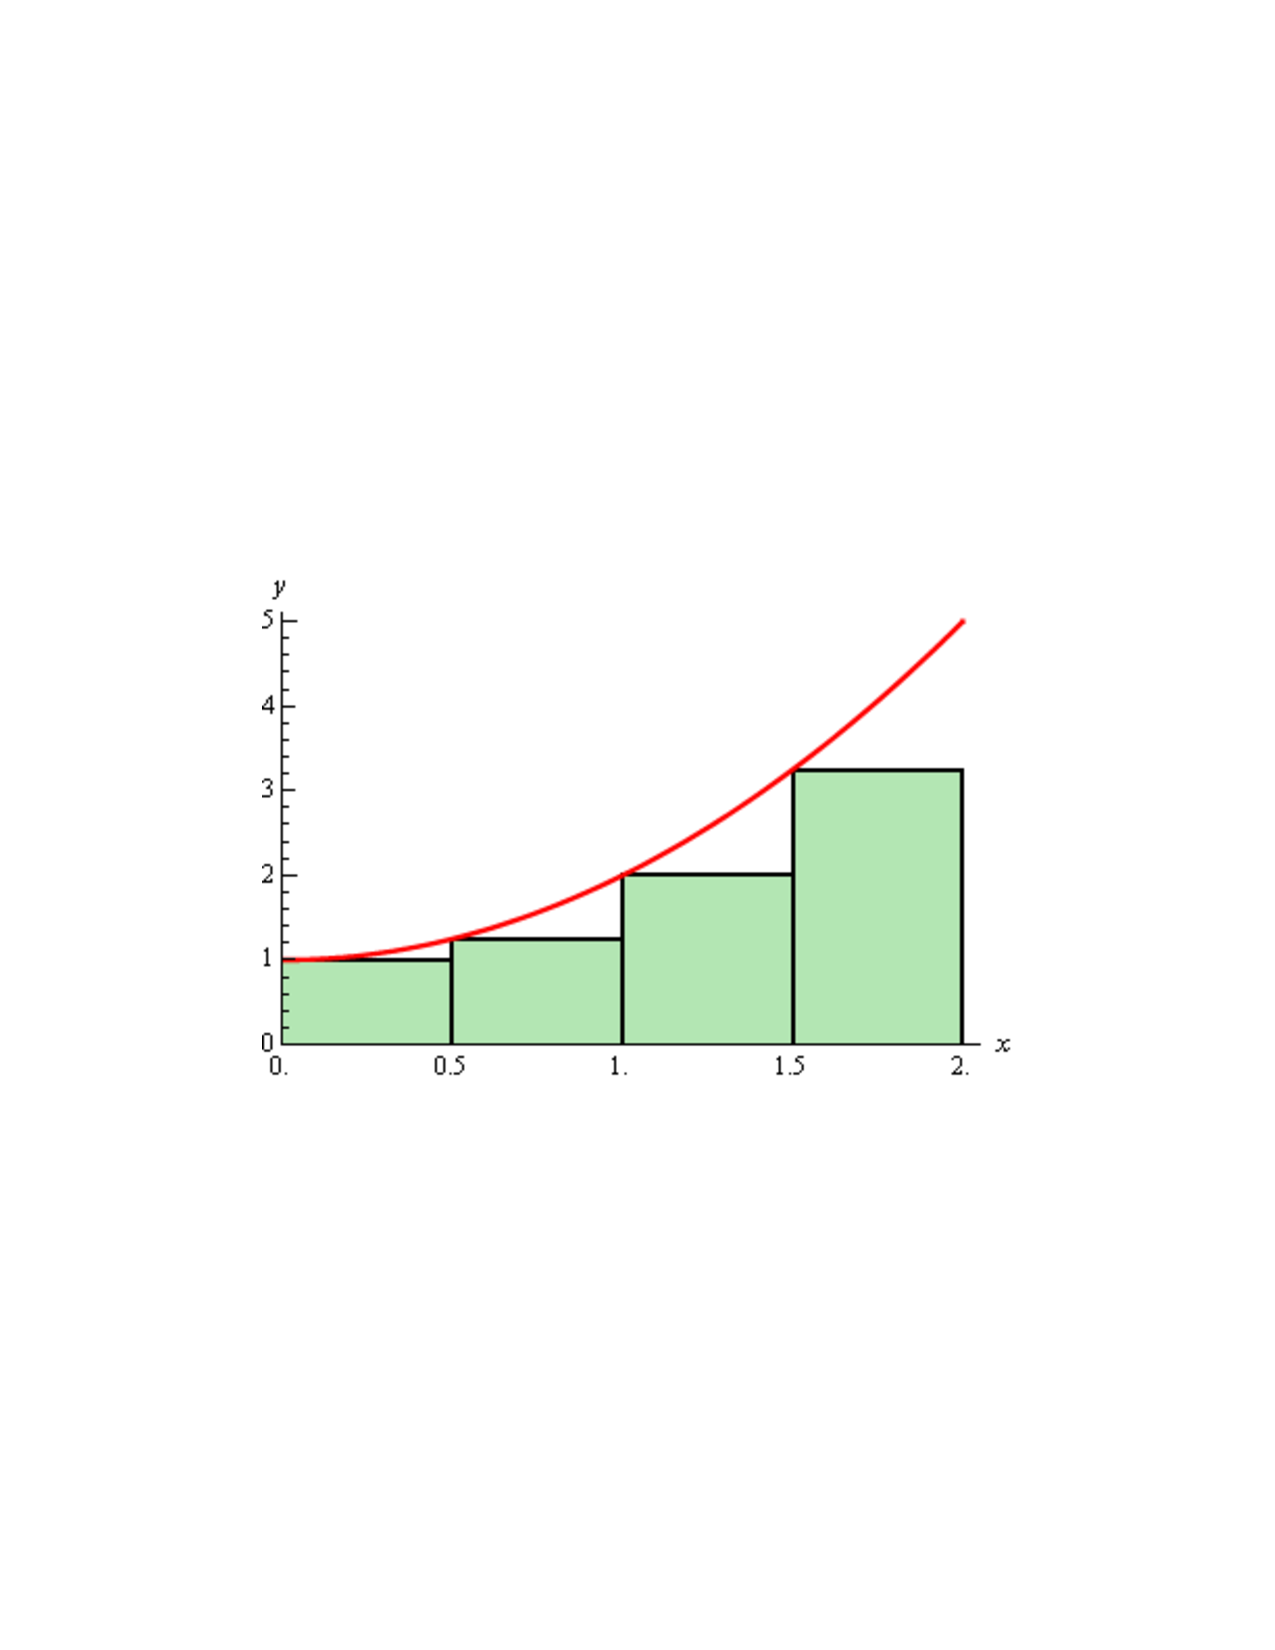
\includegraphics[scale=0.5]{img/integrals_rectangleL.pdf}\\
\end{center}
Calculate $Area(S)$.
\item Rectangle method using midpoints: \\
\begin{center}
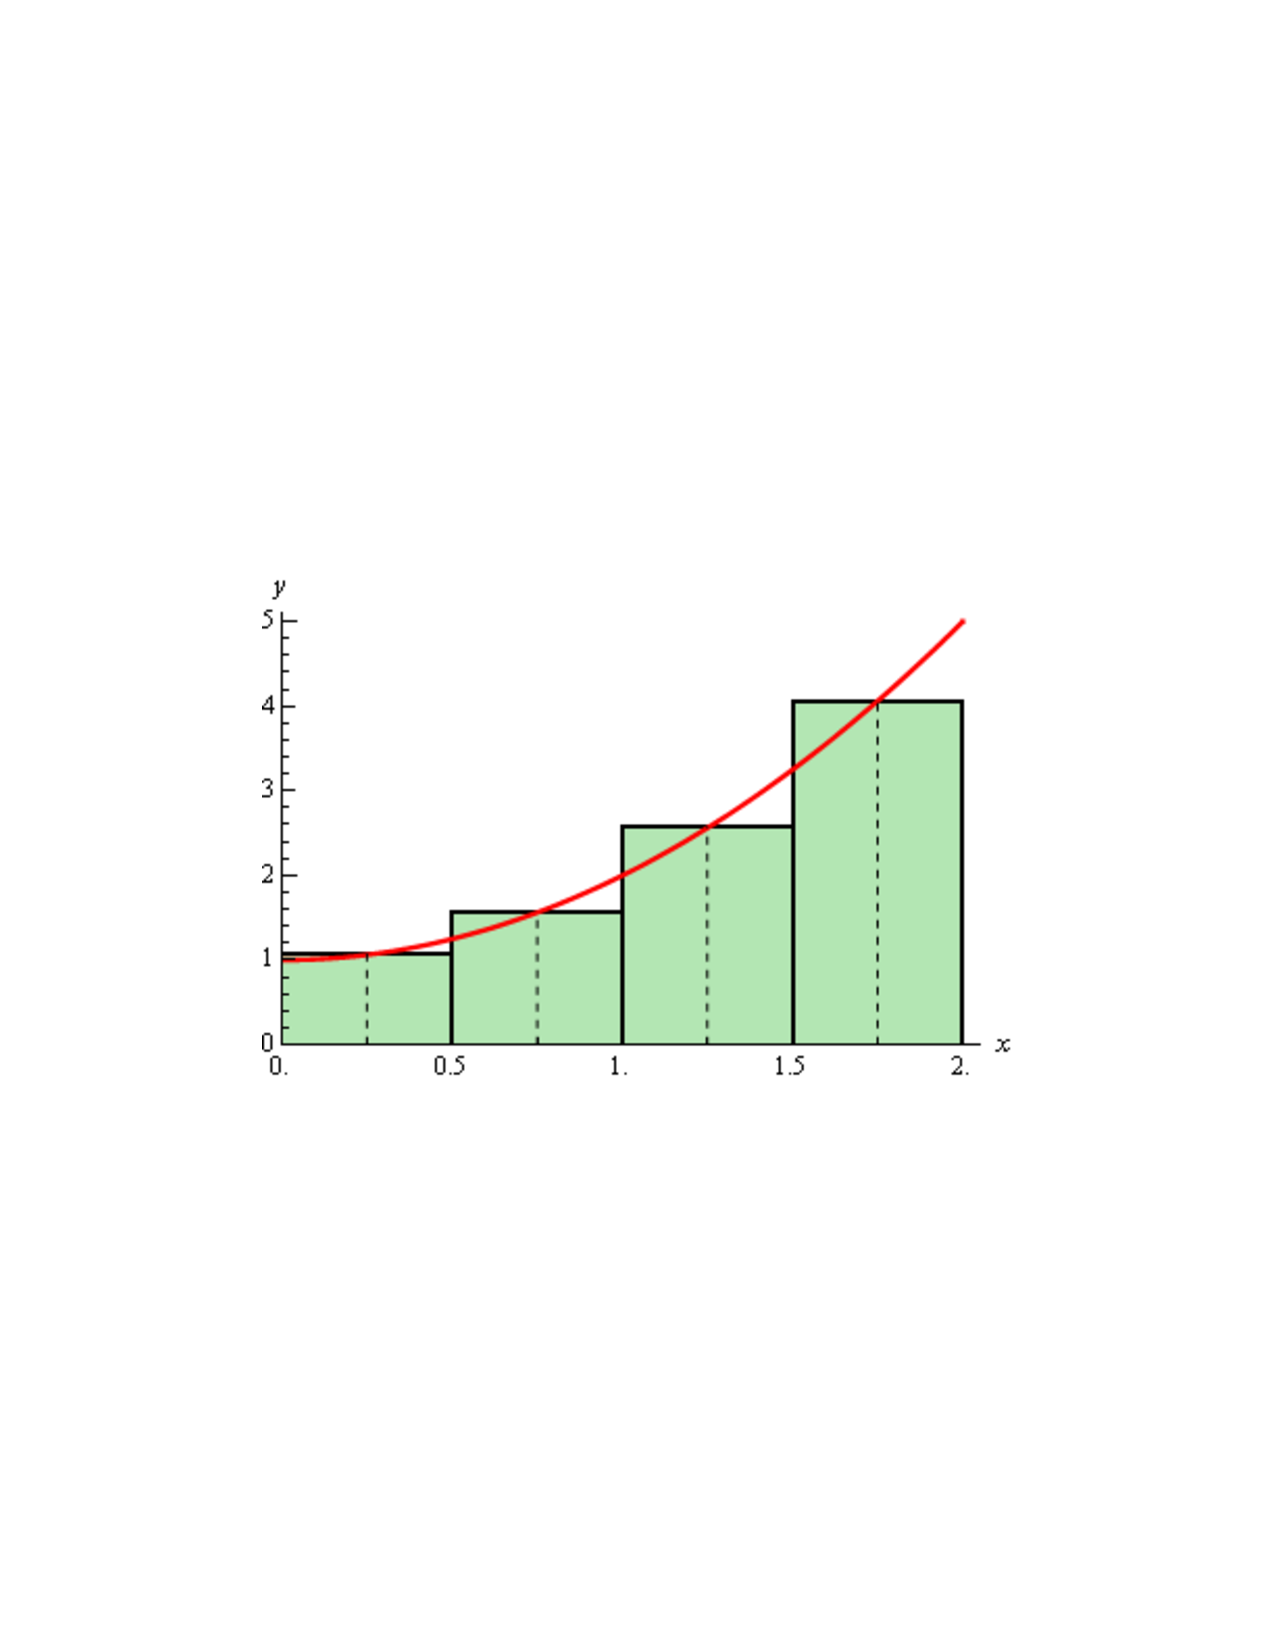
\includegraphics[scale=0.5]{img/integrals_midpoint.pdf}\\
\end{center}
Calculate $Area(S)$.
\item Which other shapes might we try?
\end{enumerate}
\item While we can use shapes like rectangles, our estimate of the area will be imprecise. One thing we might want to do is divide up our region into more parts. For example, using rectangles:
\begin{center}
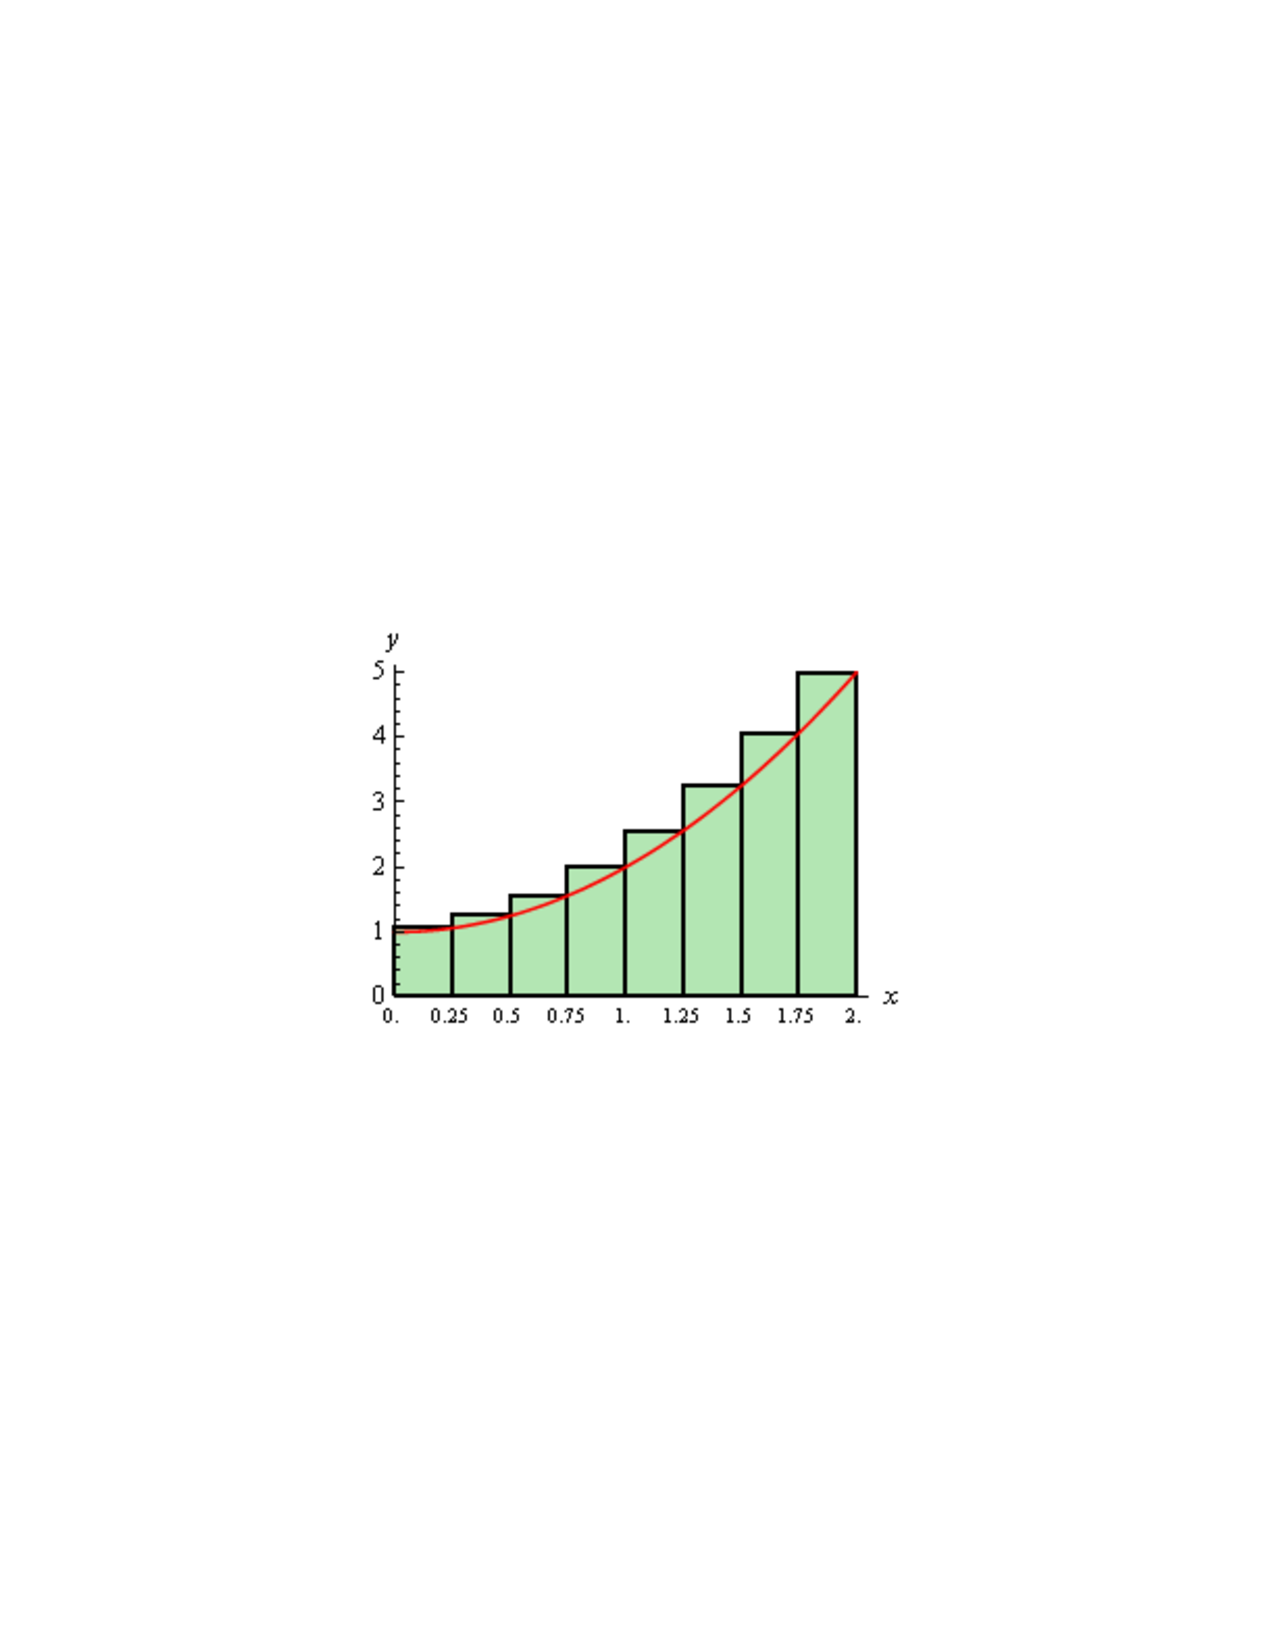
\includegraphics[scale=0.5]{img/integrals_morerectangleR.pdf}
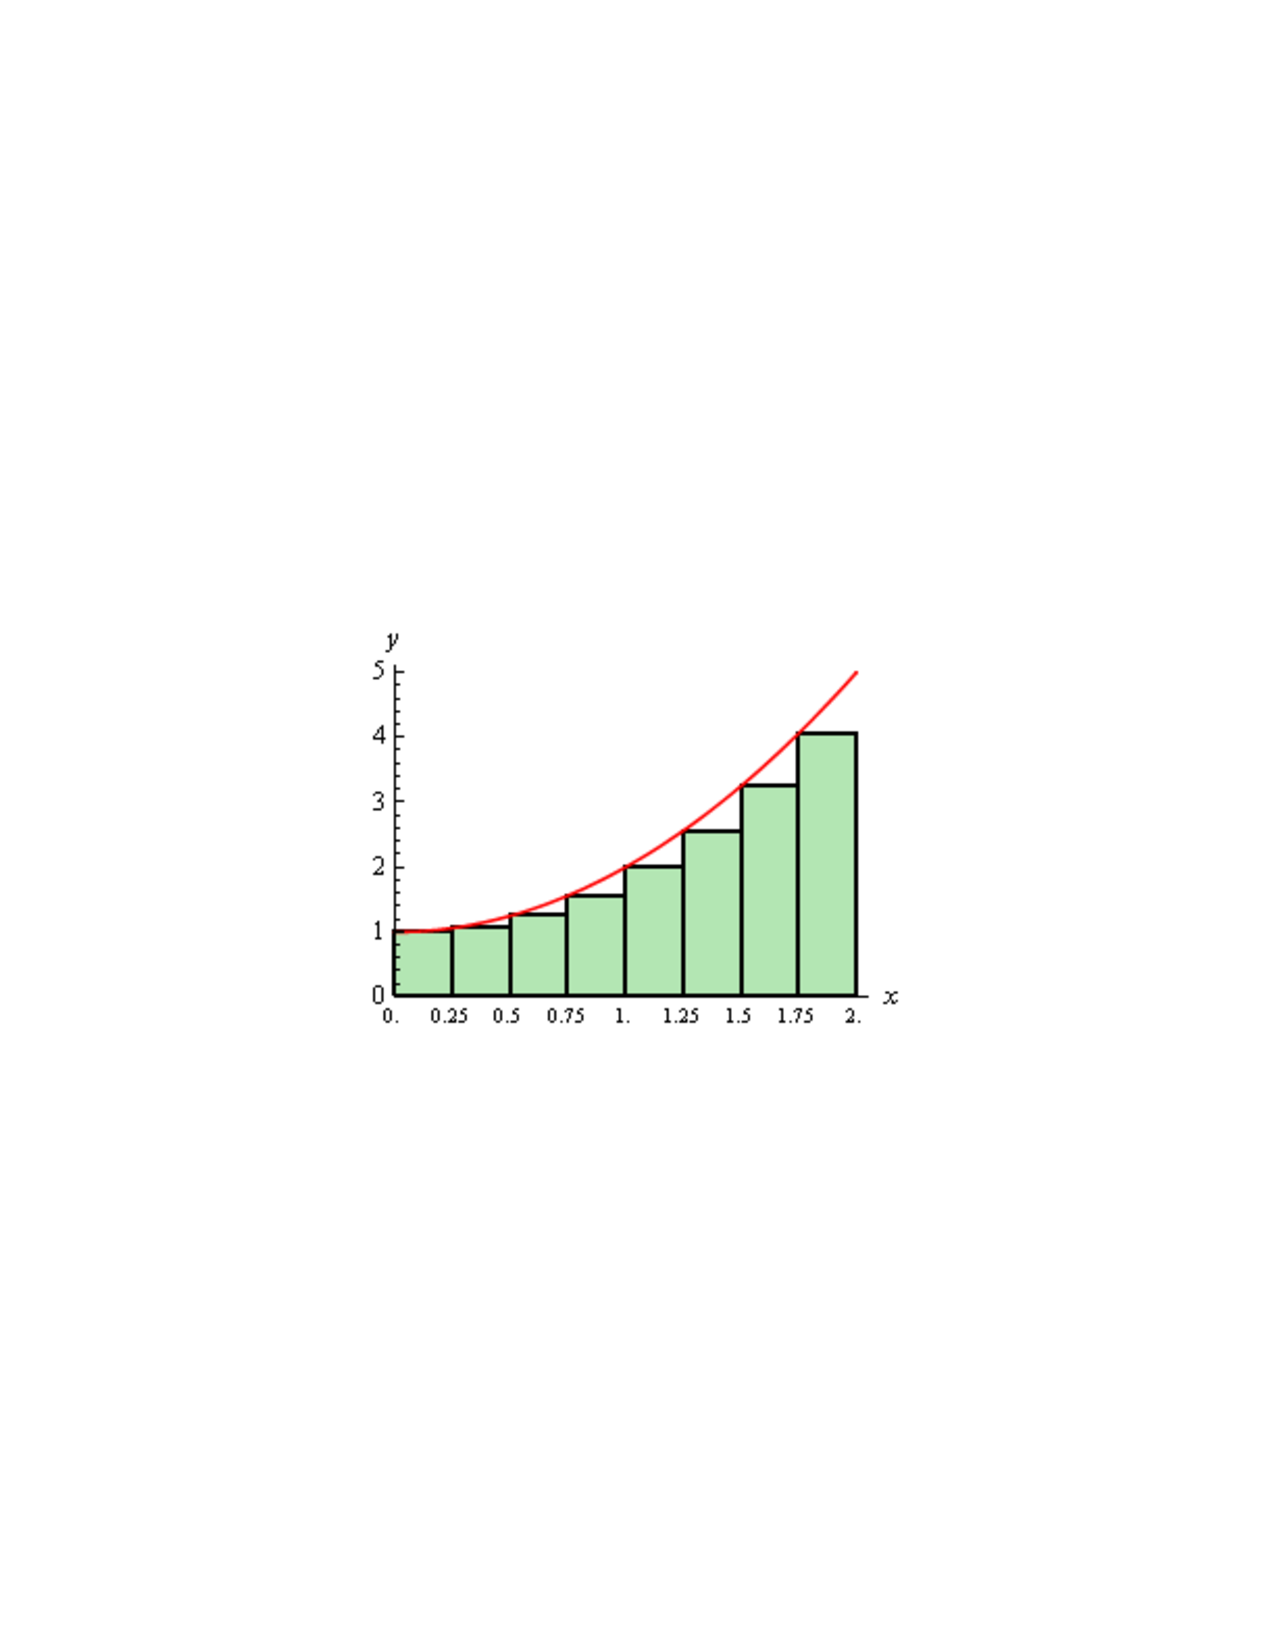
\includegraphics[scale=0.5]{img/integrals_morerectangleL.pdf}\\
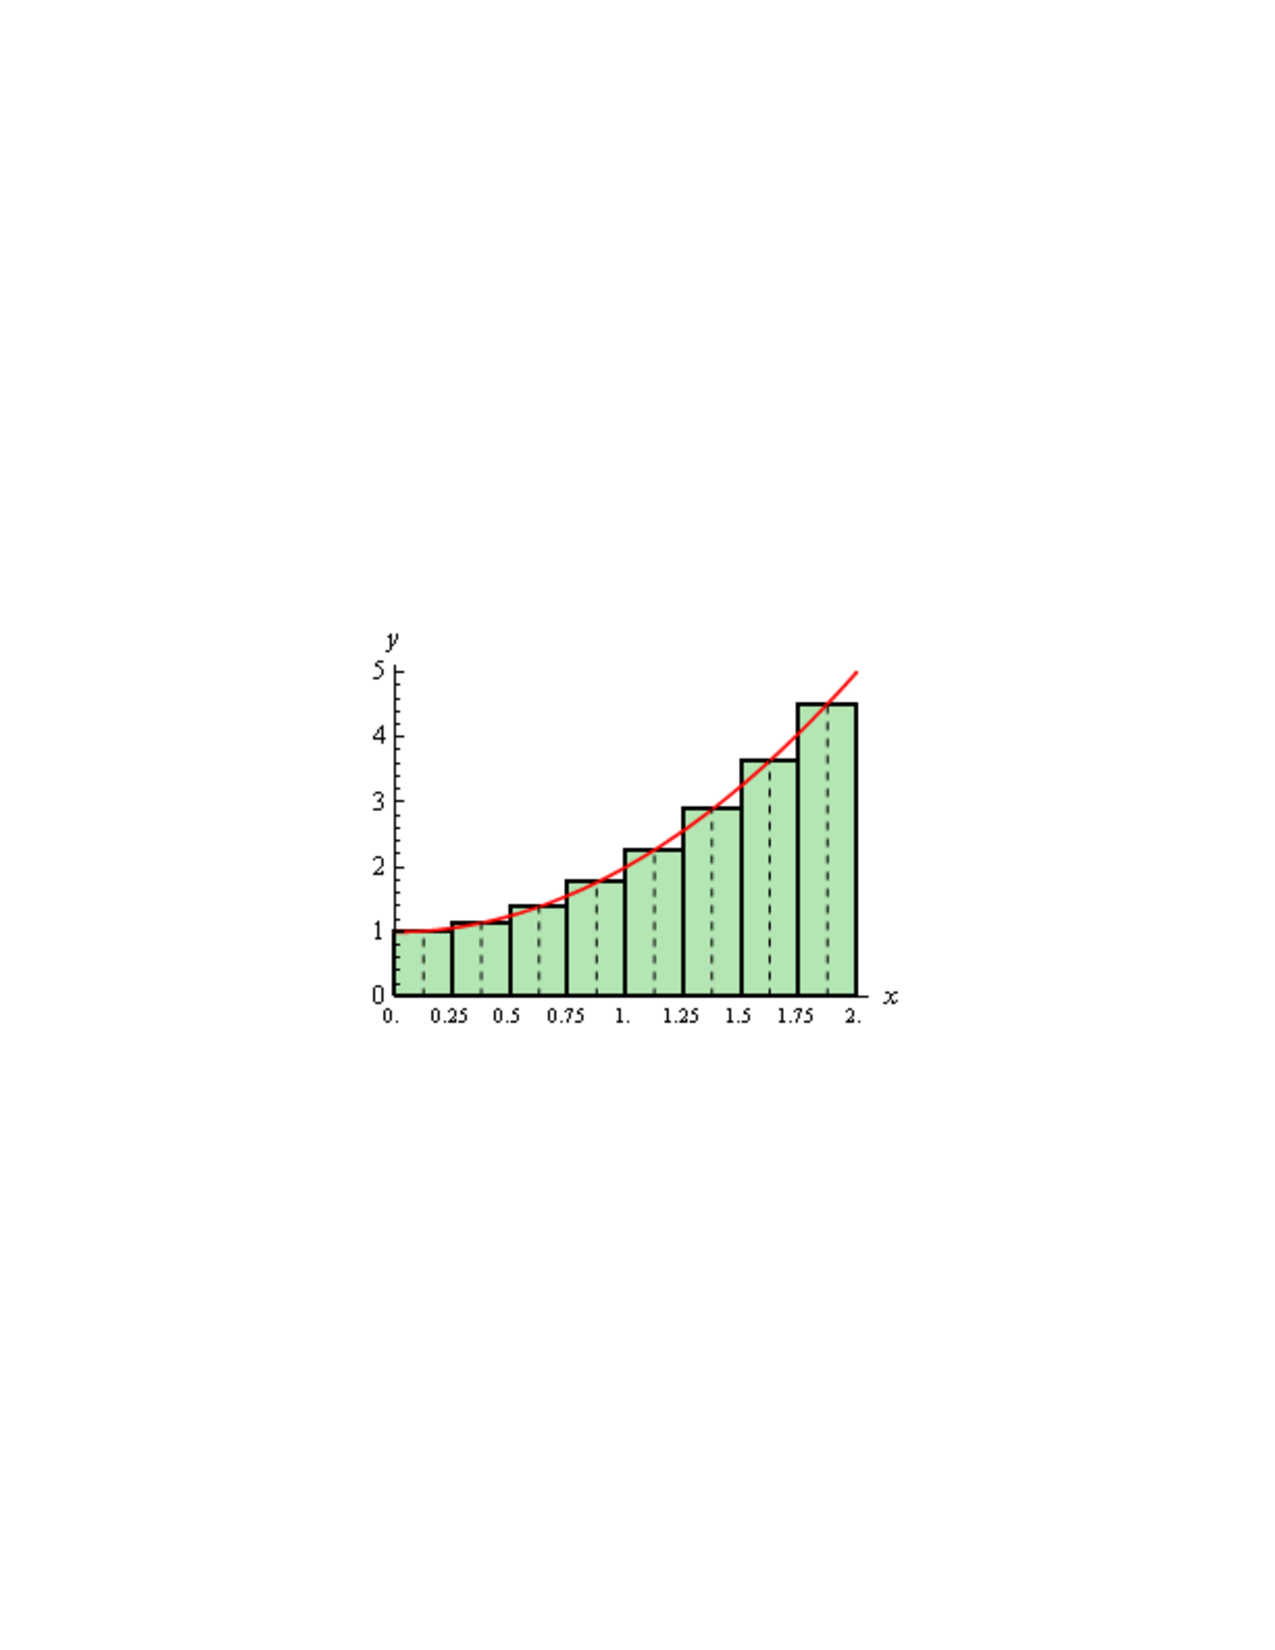
\includegraphics[scale=0.5]{img/integrals_moremidpoint.pdf}\\
\end{center}
While dividing the region may get us closer to the true answer, it is still not exact. 
\end{itemize}

\section{Indefinite Integrals: The Connection to Derivatives}
\begin{itemize}
\item We want to find a function $F$ for which $f$ is its derivative. Note that $F$ is called the \textit{antiderivative} of $f$. We can write this as:
$$
F' = f
$$
\item \textbf{Definition}: If $F$ is the antiderivative of $f$, then $F$ is called the indefinite integral of $f$:
$$
F(x) = \int f(x) \diff x 
$$
Example. Let $f(x) = 6x$. We want to find $F(x) = \int 6x \diff x$. There are many potential solutions:
\begin{enumerate}
\item $3x^2 + 1$
\item $3x^2 + 2$
\item $3x^2 + 100$, etc. 
\end{enumerate}
\textbf{IMPORTANT}: The derivative a function can have many antiderivatives. With any antiderivative, we need to add a constant $c$, unless we are told that the antiderivative passes through a particular point. 

The correct solution to our example problem, in the absence of any additional information, is $3x^2 + c$

\item \textbf{Some rules for integration}
\begin{enumerate}
\item $\displaystyle
\int [(f(x) + g(x)] \diff x = \int f(x) \diff x + \int g(x) \diff x
$
\item $\displaystyle
\int c f(x) \diff x = c \int f(x) \diff x
$
\item $\displaystyle
\int x^n \diff x = \frac{x^{n+1}}{n+1} + c
$
\item $\displaystyle
\int \frac{1}{x} \diff x = \ln|x| + c
$ 
\item $\displaystyle
\int e^x \diff x = e^x + c
$
\item $\displaystyle
\int e^{f(x)} f'(x) \diff x = e^{f(x)}+c
$
\item $\displaystyle
\int [f(x)]^nf'(x) \diff x = \frac{1}{n+1}[f(x)]^{n+1}+c
$
\item $\displaystyle
\int \frac{f'(x)}{f(x)} \diff x = \ln f(x) + c
$
\end{enumerate}
\end{itemize}

\section{Definite Integrals: Calculating the Area under a Function}
\begin{itemize}
\item We return to our initial problem of trying to calculate the area under a curve. \item Using an approximation method (i.e., one of the rectangle methods), we get close, but we want an exact answer.
\begin{itemize}
\item The rectangle approximation method is an application of a Riemann sum
$$
Area(S) = \sum_{i=1}^n \underbrace{f(x_i)}_{height} \underbrace{\Delta x}_{base}
$$
\item How above making the base of the rectangles infinitesimally small? We can use limits:
$$
Area(S) = \lim_{\Delta x\rightarrow 0} \sum_{i=1}^n \underbrace{f(x_i)}_{height} \underbrace{\Delta x}_{base}
$$
\end{itemize}
\item The Riemann Integral is the solution to our problem!
$$
\int_a^b f(x) \diff x = \lim_{\Delta x\rightarrow 0} \sum_{i=1}^n f(x_i) \Delta x
$$
\item The Riemann Integral is often referred to as the definite integral in calculus textbooks. Formally,  $\displaystyle \int_a^b f(x) \diff x$  denotes integral of function $f$ from $a$ to $b$ (or the area under curve $f(x)$ from $x=a$ to $x=b$.
\end{itemize}
\section{The Relationship Between Integration and Differentiation}
\begin{itemize}
\item \textbf{Fundamental Theorem of Calculus I (FTC I)}: If $f$ is continuous on $[a,b]$, then the function $g$ defined by 
$$
g(x) = \int_a^x f(t) \diff t \quad \text{for} \; a\leq x \leq b
$$
is an \textit{antiderivative} of $f$. 

That is, $g'(x)=f(x)$ for $a\leq x \leq b$, which can also be written as:
$$
g'(x) = \frac{\diff g(x)}{\diff x} = \frac{\diff}{\diff x}\int_a^x f(t) \diff t = f(x)
$$
when $f$ is continuous. 
\\[15pt]
Let's examine this graphically. 
\begin{itemize}
\item In the figure below, notice that $g(x)$ is the light-shaded area under the curve $f(x)$ and above the interval $[a,x]$. 
\item Also notice that $g(x+h)$ is the area under the curve $f(x)$ and above the interval $[a,x+h]$, which is represented as the area of the light shaded region plus the area of the dark shaded region. 
\item Therefore, $g(x+h) - g(x)$ is the dark shaded region under the curve $f(x)$ above the interval $[x,x+h]$. 
\item For small values of $h$, the area of the dark shaded region is \textit{approximately} equal to the area of the rectangle of height $f(x)$ with base $h$ (i.e., the area is $f(x)\cdot h$). On the figure, you can see the outline of the rectangle to which I am referring. 
\item Why is this so special? Recall the formal definition of the derivative:
$$
g'(x) = \lim_{h \rightarrow 0} \frac{g(x+h)-g(x)}{h}  
$$
We just argued that for small $h$, $g(x+h) - g(x) \approx f(x)h$.
Therefore, for small $h$,
$$
g'(x) \approx \frac{f(x)h}{h}=f(x)
$$
When we apply the limit (instead of small values of $h$), we obtain equality:
$$
g'(x) = \lim_{h \rightarrow 0} \frac{g(x+h)-g(x)}{h} = f(x) 
$$
This is quite an incredible result!
\end{itemize}
\begin{center}
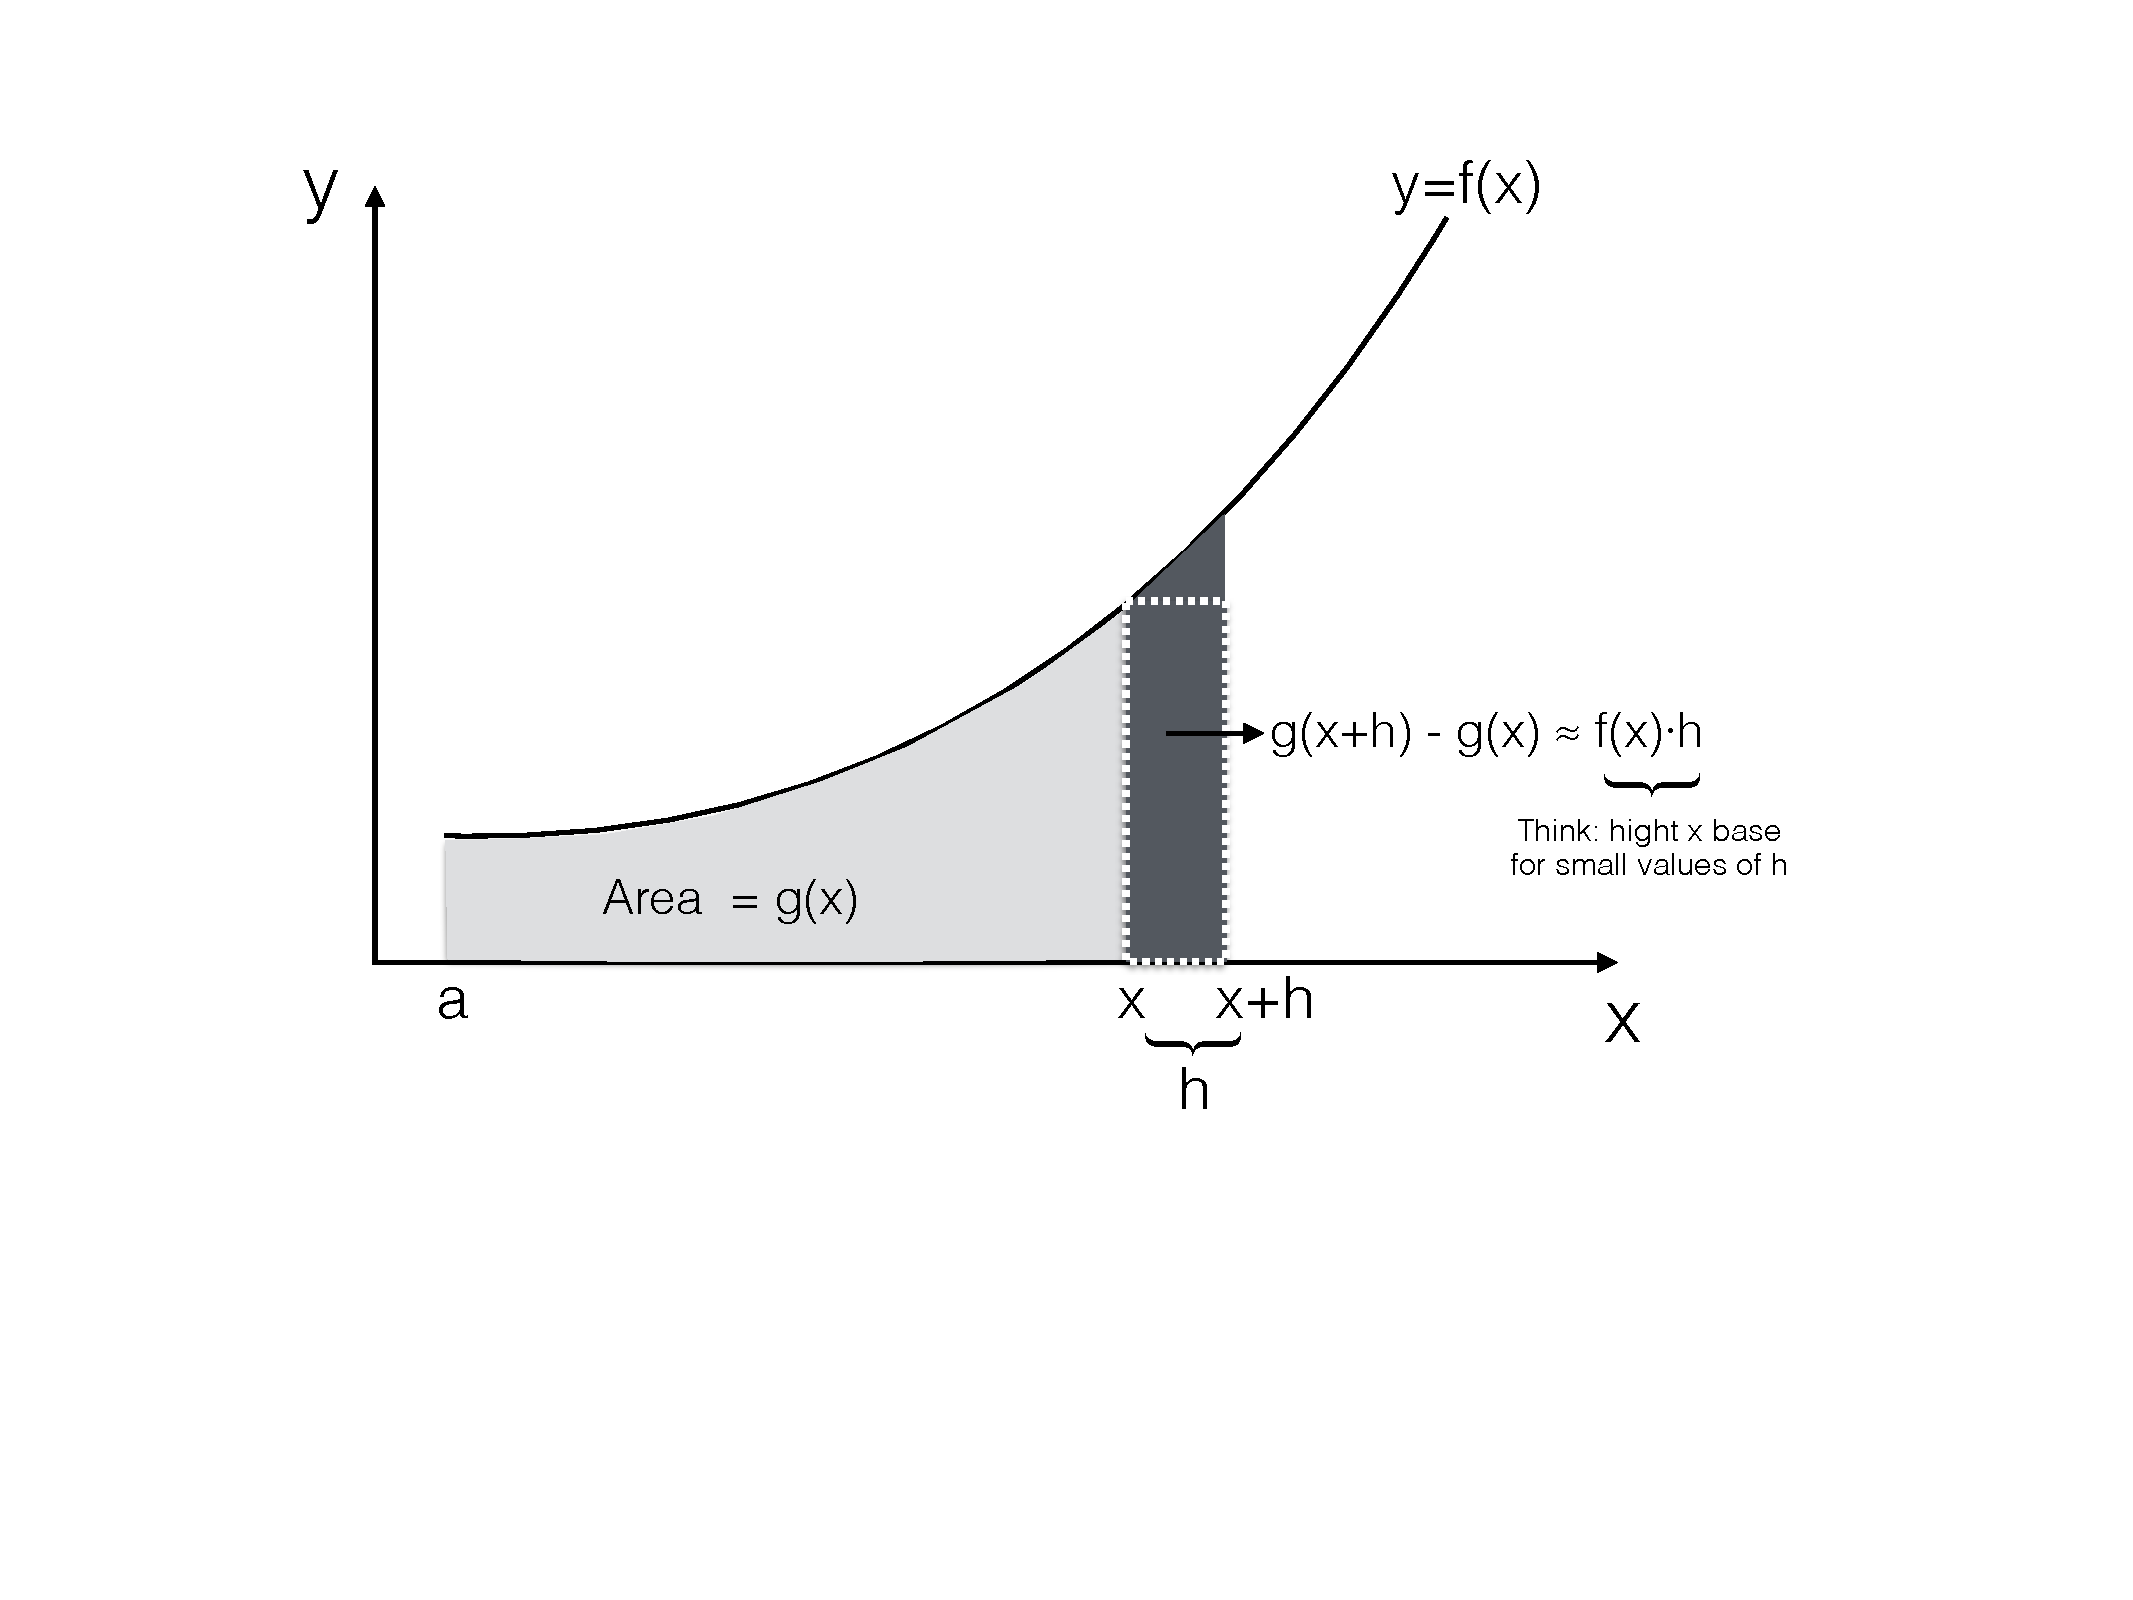
\includegraphics[scale=0.5]{img/FTC_I.pdf}
\end{center}
\item \textbf{Fundamental Theorem of Calculus II (FTC II)}: Suppose $f$ is continuous on $[a,b]$,
$$
\int_a^b f(x) \diff x = F(b) - F(a)
$$
where $F$ is any antiderivative of $f$. That is, $F' = f$. 

FTC II provides a way to calculate a definite integral:
\begin{enumerate}
\item Find the indefinite integral $F(x)$
\item Evaluate $F(b) -F(a)$
\end{enumerate}

\item \textbf{Some properties of definite integrals}
\begin{enumerate}
\item $ \displaystyle
\int_a^a f(x) \diff x = 0 \quad \text{No area under a point.}
$
\item $ \displaystyle
\int_a^b f(x) \diff x = -\int_b^a f(x) \quad \text{Switching limits changes sign of the integral}
$
\item $ \displaystyle
\int_a^b [\alpha f(x) + \beta g(x)] \diff x = \alpha \int_a^b f(x) \diff x + \beta \int_a^b g(x) \diff x
$
\item $ \displaystyle
\int_a^b f(x) \diff x + \int_b^c f(x) \diff x = \int_a^c f(x) \diff x
$
\end{enumerate}
\end{itemize}

\section{U--Substitution}
\begin{itemize}
\item Look for integral that we can write in the form:
$$
\int f(g(x))g'(x) \diff x
$$
If $F'=f$, then 
$$
\int F'(g(x))g'(x) \diff x = F(g(x)) + c
$$
\item Why? Let's examine the chain rule from differential calculus. By the chain rule, we have
$$
\frac{\diff}{\diff x}[F(g(x))] = F'(g(x))g'(x)
$$
If we make the change of variable $u = g(x)$, then we have:
\begin{align*}
\int F'(g(x))g'(x) \diff x &= F(g(x)) + c \\
&= F(u) + c \\
&= \int F'(u) \diff u 
\end{align*}
Writing $F' = f$, we get
$$
\int f(g(x))g'(x) \diff x = \int f(u) \diff u
$$
\item \textbf{Substitution Rule}: If $u=g(x)$ is a differentiable function whose image\footnote{Think of the image as the range} is an interval $I$ and $f$ is continuous on $I$, then
$$
\int f(g(x))g'(x)\diff x = \int f(u) \diff u 
$$
\item \textbf{Process}
\begin{enumerate}
\item Identify some part of $g(x)$ that might be simplified by substituting in a single variable $u$, which will then be a function of $x$.
\item Determine if $g(x) \diff x$ can be reformulated in terms of $u$ and $\diff u$
\item Solve the indefinite integral
\item Substitute back in for $x$
\end{enumerate}
\item \textbf{Process for definite integrals}: Using the procedure above,
$$
\int_a^b g(x) \diff x = \int_c^d f(u) \diff u = F(d) - F(c)
$$
where $c=u(a)$ and $d=u(b)$.
\end{itemize}

\section{Integration by Parts}
\begin{itemize}
\item Recall the product rule for differentiation:
$$
\frac{\diff}{\diff x}[f(x)g(x)] = f(x)g'(x) + g(x)f'(x)
$$
Taking the integral of both sides of the equation, we obtain:
$$
f(x)g(x) = \int f(x)g'(x) \diff x + \int g(x)f'(x) \diff 
$$
Rearranging terms, we obtain the familiar form for integration by parts:
$$
\int \underbrace{f(x)}_{u}\underbrace{g'(x) \diff x}_{\diff v} = \underbrace{f(x)}_{u}\underbrace{g(x)}_v - \int \underbrace{g(x)}_v \underbrace{f'(x) \diff x}_{\diff u}
$$
Most people remember the integration by parts formula as:
$$
\int u \diff v  = uv - \int v \diff u 
$$
where $\diff u = u'(x)\diff x$ and $\diff v = v'(x) \diff x$
\item For definite integrals, we have
$$
\int_a^b f(x)g'(x) \diff  x = f(x)g(x)\big |_a^b - \int_a^b g(x)f'(x) \diff x
$$
\item The goal is to obtain a simpler integral than one we started with. HINT: Choose $u=f(x)$ to be a function that becomes simpler when differentiated (or at least not more complicated) as long as $\diff v = g'(x) \diff x$ can be readily integrated to give $v$.
\end{itemize}

\newpage
\section{Improper Integrals (Infinite Intervals)}

\begin{itemize}

\item \textbf{Definitions of Improper Integrals}
\begin{enumerate}[(a)]
\item If $\displaystyle \int_a^t f(x) \diff x$ exists for every number $t\geq a$, then
$$
\int_a^\infty f(x) \diff x = \lim_{t \rightarrow \infty} \int_a^t f(x) \diff x
$$
provided the limit exists as a finite number. 
\item If $\displaystyle \int_t^b f(x) \diff x $ exists for every number $t \leq b$, then 
$$
\int_{-\infty}^b f(x) \diff x = \lim_{t \rightarrow -\infty} \int_t^b f(x) \diff x
$$
provided this limit exists as a finite number.
\end{enumerate}
\item The improper integrals in (a) and (b) are called \textbf{convergent} if the corresponding limit exists and \textbf{divergent} if it does not exist.
\item If both $\displaystyle \int_a^\infty f(x) \diff x$ and $\displaystyle \int_{-\infty}^a f(x) \diff x$ are \textbf{convergent}, then we define
$$
\int_{-\infty}^{\infty} f(x) \diff x = \int_{-\infty}^a f(x) \diff x + \int_a^\infty f(x) \diff x
$$
where $a$ is any real number.
\item Useful reminder: \textbf{L'Hospital's Rule}. 
\begin{itemize}
\item Why do we use it? To figure out the limits of functions that are in an \textbf{indeterminate} form. For example, suppose we want to find the limit of the form
$$
\lim_{x\rightarrow a}\frac{f(x)}{g(x)}
$$
where both $f(x) \rightarrow 0$ and $g(x) \rightarrow 0$ as $x \rightarrow a$, then the limit may or may not exist. Essentially, you get the indeterminate form $\frac{0}{0}$. 

Or suppose you have a limit of the form 
$$
\lim_{x\rightarrow a}\frac{f(x)}{g(x)}
$$
where both $f(x) \rightarrow \infty$ and $g(x) \rightarrow \infty$ as $x \rightarrow a$, then the limit may or may not exist. Essentially, you get the indeterminate form $\frac{\infty}{\infty}$. 
\item Statement of \textbf{L'Hospital's Rule}: Suppose $f$ and $g$ are differentiable and $g'(x)\neq 0$ near $a$ (except possibly at $a$.) Suppose that
\begin{enumerate}
\item $\lim_{x\rightarrow a} f(x) = 0$ and $\lim_{x\rightarrow a} g(x) = 0$ \quad \textbf{OR} 
\item $\lim_{x\rightarrow a} f(x) = \pm \infty$ and $\lim_{x\rightarrow a} g(x) = \pm \infty$
\end{enumerate}
Then
$$
\lim_{x\rightarrow a}\frac{f(x)}{g(x)} = \lim_{x\rightarrow a}\frac{f'(x)}{g'(x)}
$$
if the limit on the right side exists or is $\infty$ or $-\infty$. 
\end{itemize}
\end{itemize}


\end{document}
\bibliography{mathcamp}
